\section{Propuesta de solución}
\label{sec:propuesta}

Para abordar la clasificación de transacciones financieras, se ha desarrollado un pipeline modular que abarca desde el preprocesamiento de texto hasta la evaluación de múltiples modelos de aprendizaje supervisado.

\subsection{Dataset Unificado y Preprocesamiento}
Después de hacer tests con el dataset original, nos dimos cuenta de que no era suficiente para entrenar un modelo de machine learning, por lo que decidimos combinarlo con el dataset modificado. Aun así, al ser datasets tan diferentes, no evaluaban corréctamente el resto de categorías, por lo que decidimos quedarnos solo con el dataset modificado.

Se han combinado dos fuentes de datos principales: \texttt{db\_orig.csv} y \newline \texttt{db\_modified\_descriptions.csv}, creando un corpus robusto con el doble de ejemplos por categoría y que ha funcionado mejor. Pero la diferencia era demasiado grande y aunque ajustaba mejor decidimos supervisar y depurar la creación de descripciones creando la base de datos \texttt{db\_mod\_descript.csv} que ha mejorado aún más las predicciones. Recordando la importancia que se habló en la primera práctica sobre la gran importancia de la creación y depuración de datos en los problemas que estamos afrontando.
\newline El preprocesamiento incluye:
\begin{itemize}
    \item Conversión a minúsculas y eliminación de caracteres especiales.
    \item Vectorización de texto mediante \textbf{TF-IDF} (\textit{Term Frequency - Inverse Document Frequency}) para transformar las descripciones en representaciones numéricas.
\end{itemize}

\subsection{Comparativa de Modelos}
Se evaluaron cuatro arquitecturas distintas mediante una validación con partición 50/50 para asegurar la capacidad de generalización:
\begin{itemize}
    \item \textbf{Logistic Regression}: Proporcionó alta explicabilidad pero rendimiento ligeramente inferior en clases minoritarias.
    \item \textbf{SGDClassifier}: El modelo base del sistema, destaca por su extrema eficiencia en recursos.
    \item \textbf{Random Forest}: Elevada precisión, pero con un coste computacional y de almacenamiento excesivo para el dominio del problema.
    \item \textbf{Linear SVM}: El modelo con mejor rendimiento global.
\end{itemize}

\newpage
\subsection{Resultados y Selección Final}

%  Añadir imagen gráfica
\begin{figure}[h]
    \centering
    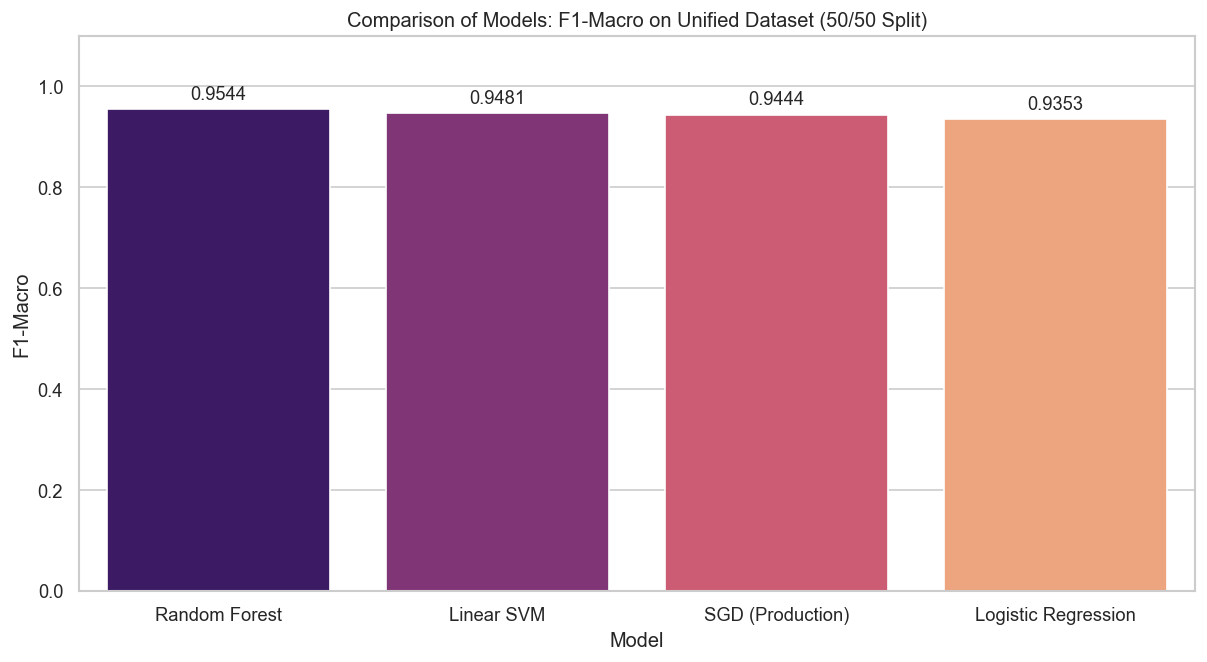
\includegraphics[width=0.8\textwidth]{figures/comparation_models.png}
    \caption{Resultados de la comparativa con el dataset conjunto}
    \label{fig:comparation_models}
\end{figure}

Tras las pruebas, el modelo \textbf{Linear SVM} obtuvo un \textbf{F1-Macro de 0.9481} con el dataset unificado \ref{fig:comparation_models} y \textbf{F1-Macro de 1} con el dataset modificado y revisado, superando al SGD original. Este modelo ofrece el mejor equilibrio entre:
\begin{enumerate}
    \item \textbf{Precisión}: Máxima eficacia en la separación de categorías complejas (como ``Ocio'' vs ``Ocio, Vacaciones'').
    \item \textbf{Explicabilidad}: Al ser un modelo lineal, permite auditar los pesos de las palabras clave.
    \item \textbf{Eficiencia}: Mantiene una huella de memoria ligera y tiempos de inferencia casi instantáneos.
\end{enumerate}




Por tanto, se ha seleccionado \texttt{LinearSVM.joblib} como el modelo principal para la implementación en el sistema de producción.
